\documentclass[11pt]{beamer}


% ===== Packages =====
\usepackage[utf8]{inputenc}
\usepackage[T1]{fontenc}

\usepackage{graphicx}
\usepackage{tikz}

\usepackage[backend=biber, autolang=other, style=phys, sorting=none]{biblatex}  % Citing
\addbibresource{../bibliography/bibliography.bib}

% ===== Typeface =====
\usepackage[sfdefault]{FiraSans} % !
% \usepackage{helvet}
% \usepackage[sfdefault]{AlegreyaSans}
% \usepackage[sfdefault]{plex-sans} % !
% \usepackage{avant}
% \usepackage{montserrat}
% \usepackage{raleway}

% ===== Beamer theme =====
\usetheme{Boadilla} % other interesting built-in: Boadilla, CambridgeUS (if we want sections in header), Pittsburgh (super-plain)

% \useoutertheme{infolines} % Alternatively: miniframes, infolines, split
\useinnertheme{circles}

\setbeamertemplate{blocks}[rounded][shadow=false]
\setbeamertemplate{navigation symbols}{}

% ===== Colors =====
% \usecolortheme{beaver}
\definecolor{UBCblue}{rgb}{0.04706, 0.13725, 0.26667} % UBC Blue (primary)
\usecolortheme[named=UBCblue]{structure}

% \setbeamercolor{block title}{bg=cyan!50, fg=white} % modifying colors (the ! is for trasparency)
% \definecolor{darkred}{rgb}{0.8,0,0}

% \setbeamercolor{section in toc}{fg=black,bg=white}
% \setbeamercolor{alerted text}{fg=darkred!80!gray}
% \setbeamercolor*{palette primary}{fg=darkred!60!black,bg=gray!30!white}
% \setbeamercolor*{palette secondary}{fg=darkred!70!black,bg=gray!15!white}
% \setbeamercolor*{palette tertiary}{bg=darkred!80!black,fg=gray!10!white}
% \setbeamercolor*{palette quaternary}{fg=darkred,bg=gray!5!white}

% \setbeamercolor*{sidebar}{fg=darkred,bg=gray!15!white}

% \setbeamercolor*{palette sidebar primary}{fg=darkred!10!black}
% \setbeamercolor*{palette sidebar secondary}{fg=white}
% \setbeamercolor*{palette sidebar tertiary}{fg=darkred!50!black}
% \setbeamercolor*{palette sidebar quaternary}{fg=gray!10!white}

% \setbeamercolor*{titlelike}{parent=palette primary}
% \setbeamercolor{titlelike}{parent=palette primary,fg=darkred}
% \setbeamercolor{frametitle}{bg=gray!10!white}
% \setbeamercolor{frametitle right}{bg=gray!60!white}

% \setbeamercolor*{separation line}{}
% \setbeamercolor*{fine separation line}{}

% \definecolor{cyanish}{RGB}{10,250,250}  % different ways to define colors
% \definecolor{lightgreen}{HTML}{CCFF99}
% \definecolor{orangish}{wave}{620}
% \colorlet{ochre}{blue!30!yellow!70!}

% ===== Text properties =====
\renewcommand*\familydefault{\sfdefault}
% \linespread{1.3} % Change line spacing
\usefonttheme{professionalfonts}
\setbeamerfont{bibliography entry author}{size=\scriptsize, series=\normalfont} 
\setbeamerfont{bibliography entry title}{size=\scriptsize, series=\bfseries} 
\setbeamerfont{bibliography entry location}{size=\scriptsize, series=\normalfont} 

% ===== Global background =====
% %Global Background must be put in preamble
% \usebackgroundtemplate%
% {%
%     \includegraphics[width=\paperwidth,height=\paperheight]{newton.jpg}%
% }

% ===== Title logo =====
\titlegraphic { 
\begin{tikzpicture}[overlay,remember picture]
\node[right=0.2cm] at (current page.147){
    
\includegraphics[width=1.5cm]{../figures/EPFL_logo.png}
};
\end{tikzpicture}
}
% Or more simply:
% \titlegraphic{
\includegraphics[width=1.5cm]{../figures/EPFL_logo.png}} % Title logo

% ===== Presentation =====
\title[(À enlever)]{Argon plasma analysis using Langmuir probes}
\author[Tom Vadot \and Matteo Veneziano]{Tom Vadot \and Matteo Veneziano}
\institute[]{EPFL Section of Physics}
\date{November 29, 2024}
% \logo{
\includegraphics[width=1.5cm]{../figures/EPFL_logo.png}} % logo en chaque page

\begin{document}

\begin{frame}
    \titlepage
\end{frame}

\begin{frame}{Defining plasma}{Maybe split in the middle between quasineutral and collective behaviour?}
    "A \emph{quasineutral} gas of charged and neutral particles which exhibit \emph{collective} behaviour" \footfullcite{chen_introduction_2006}

    Quasineutrality: even though the particles making up a plasma consist of free electrons and ions, their overall charge densities cancel each other in equilibrium \footfullcite{gibbon_introduction_2016}

    Collective behaviour: macroscopic fields dominate over short-lived microscopic fluctuations

\end{frame}


\begin{frame}{Langmuir probes}

\end{frame}


\begin{frame}{The $I$--$V$ characteristic curve}
    
\end{frame}


\begin{frame}{Ion acustic waves}
    
\end{frame}


\begin{frame}{Experimental setup}
    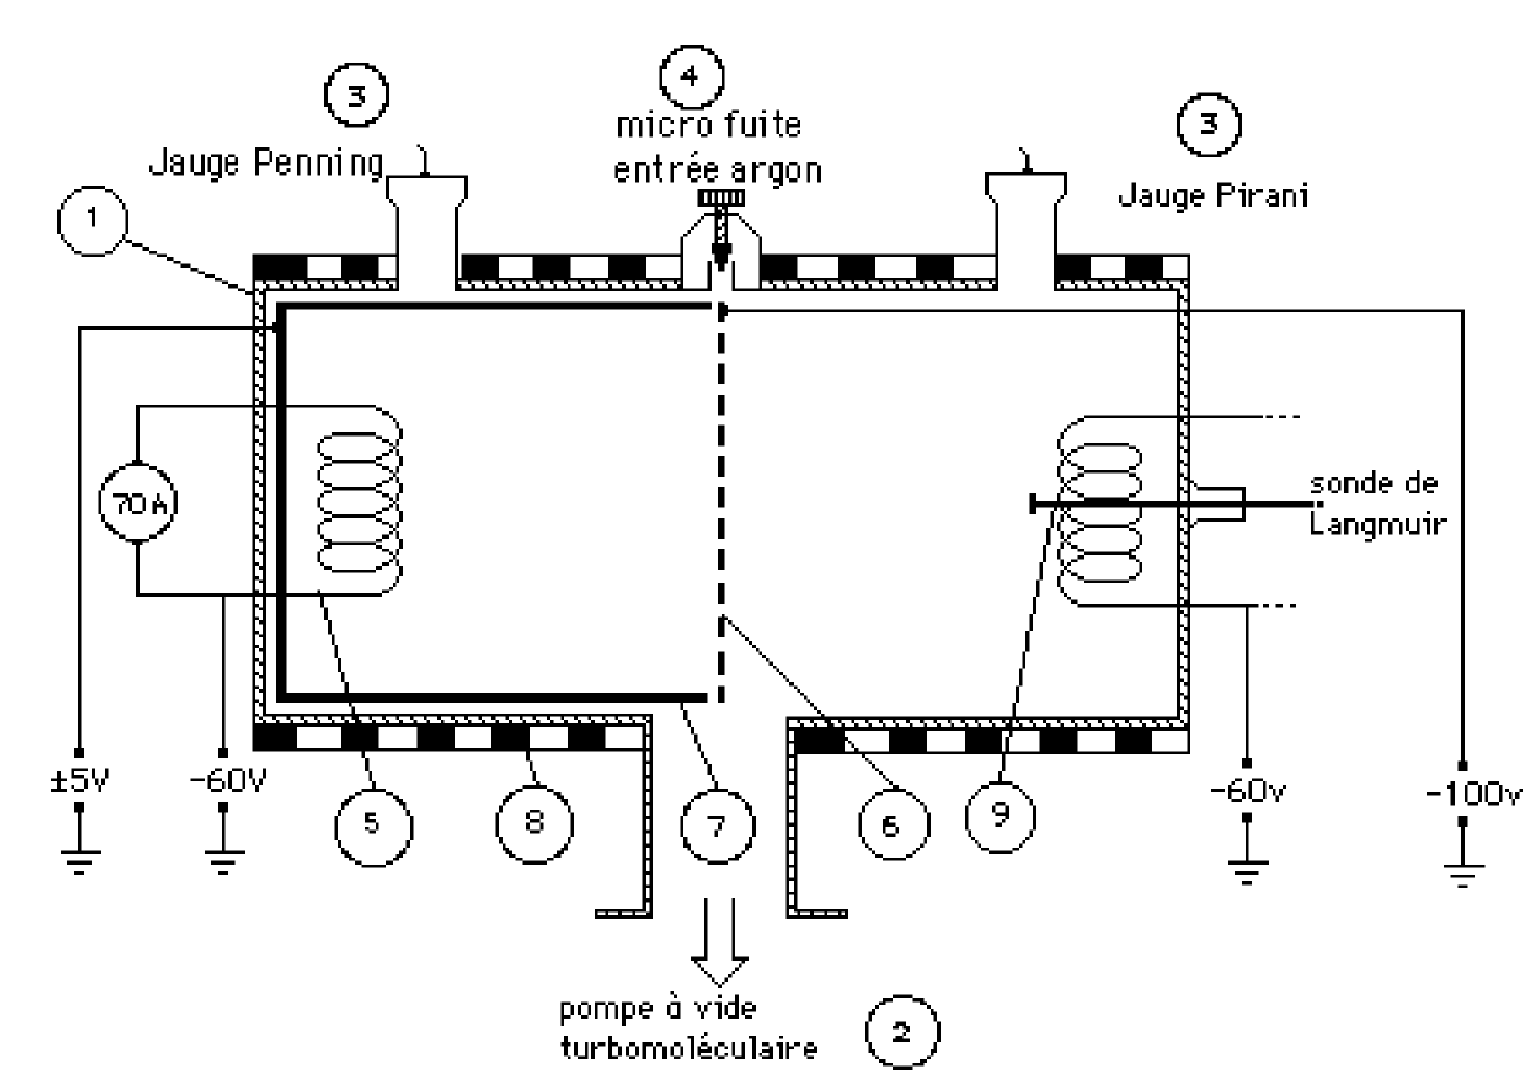
\includegraphics[width=6cm]{../figures/experimental-setup.png}
\end{frame}


\begin{frame}{(Variation avec position, differentes pressions)}{Mise en page en dernier, avant écrire les phrases}
    \begin{columns}
        \column{0.5\textwidth}
        [Observations]

        \column{0.5\textwidth}
        \centering
        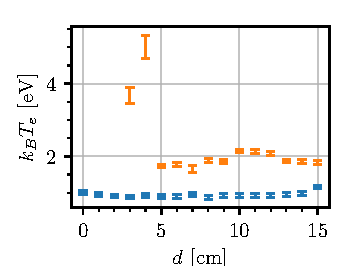
\includegraphics[width=\textwidth]{../figures/temperatureeV_position.pdf}
        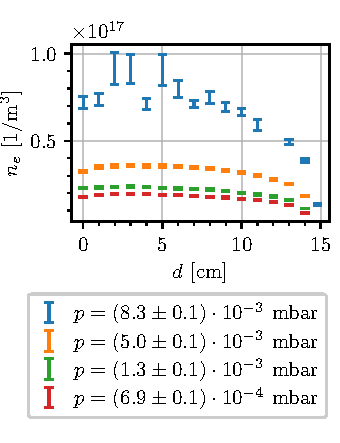
\includegraphics[width=\textwidth]{../figures/density_position.pdf}
    \end{columns}
\end{frame}
    
\begin{frame}{Some other stuff about Plasma}
    \begin{columns}[T]
        \column{0.6\textwidth}
        \centering
        This is column one with 75\% text width.

        \column{0.4\textwidth}
        \centering
        This is column two with 25\% text width.
        % \vspace{5cm}
        % And something in the bottom right corner.
    \end{columns}
\end{frame}

\begin{frame}{Some other stuff about Plasma}{Now with lines!}
    \begin{columns}
    % Column 1
    \begin{column}{0.49\textwidth}
        \begin{itemize}
            \item Mmmh yes the plasma is made of plasma
            \item Second smart remark
            \item Third smart remark
        \end{itemize}
    \end{column}
   % Column 2 (vertical line)
    \begin{column}{.02\textwidth}
        \rule{.1mm}{0.7\textheight}
    \end{column}
   % Column 3    
    \begin{column}{0.49\textwidth}
        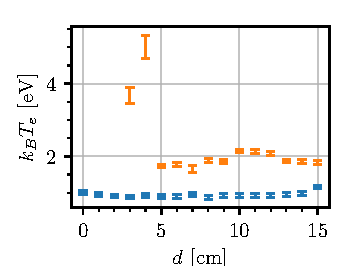
\includegraphics[width=\textwidth]{../figures/temperatureeV_position.pdf}
    \end{column}
    \end{columns}
\end{frame}

\begin{frame}{On the thermal properties of plasma}
    \begin{block}{Caution!}
        Plasma is hot
    \end{block}
\end{frame}

\begin{frame}{Overlays in Beamer}
    The easiest way is to use the stop command
    \pause

    Like this
    \pause

    There are other very customisable ways but we won't need them.
\end{frame}

\end{document}